\section{Direct lattice}

\vspace*{0.5cm}
\begin{center}
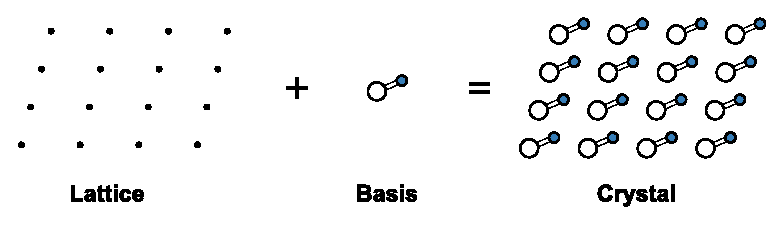
\includegraphics[width=0.75\textwidth]{crystal_structure/figures/crystal.eps}
\end{center}

\noindent
The mathematical description of the crystal consists of two parts: the \emph{lattice} which is a periodic grid of points extending over space and the \emph{basis} which in this context is the set of ions repeating at every lattice point.

The lattice can be described by the set of so called \emph{lattice vectors} $\lbrace\mathbf{R}\rbrace$ given by
\begin{equation}\label{eq:direct_lattice}
\mathbf{R} \equiv \mathbf{R}_{n_1 n_2 n_3}  = n_1 \mathbf{a}_1 + n_2 \mathbf{a}_2 + n_3 \mathbf{a}_3,
\end{equation}
where $n_i \in \mathds{Z}$ and $\mathbf{a}_i$ are linearly independent vectors in the real space called the \emph{primitive vectors}. The primitive vectors have the dimensions of length owing to which the lattice spanned by them is referred to as the \emph{direct lattice}. It should be noted the choice of the primitive vectors is not unique; any non-collinear set of the lattice vectors can be used.

The lattice can be infinite or finite depending on the allowed values of $n_i$. Quite often it is convenient to deal with infinite lattice which extends over all spatial dimensions. In such case the lattice is known as the \emph{Bravais lattice}. 

An important concept of \emph{unit cell} builds upon the lattice. A unit cell is a volume of space that can fill the entire space without overlaps or leaving gaps behind when translated by a suitable set of Bravais lattice vectors. A \emph{primitive unit cell} is a special set of unit cells which enclose precisely one lattice point. Therefore, if the number density of lattice points is $n$, the primitive unit cell volume $v$ is 
\begin{equation}
v = \frac{1}{n}
\end{equation}
regardless the shape of the cell. Sometimes it is, however, easier to work with a \emph{conventional unit cell} instead. For example, a primitive unit cells of a BCC (body-centered cubic) lattice can be difficult to work with since their angles are not orthogonal. The usual choice is to use a cubical cell containing two lattice points instead. Note that whereas primitive unit cells can be translated by all the lattice vectors without any overlaps, the same is not true for the conventional ones. 

There is, however, a common used way to choose a primitive unit cell that has the full symmetry of the lattice. Consider a single lattice point and take all the points in its vicinity that are nearer to it than any other point in the lattice. The volume covered by those points leads to a unique primitive unit cell which is known as the \emph{Wigner-Seitz cell}. The concept is worth remembering as it has an important role in the subsequent discussion.

\vspace*{0.5cm}
\begin{figure}[h!]
\centering
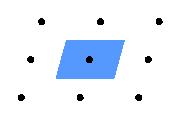
\includegraphics[width=0.4\textwidth]{crystal_structure/figures/wigner-seitz.eps}
\caption{Wigner-Seitz cell of an oblique 2D-lattice. The blue area covers the points closest to the lattice point in the center.}
\end{figure}

\section{Reciprocal Lattice}
In the scope of this for a general plane wave in terms of position $\mathbf{r}$ and time $t$ is written as
\begin{equation}
f(\mathbf{r},t) = A e^{i\mathbf{k}\cdot\mathbf{r} - i\omega t}.
\end{equation}
The wavevector $\mathbf{k}$ points at the direction of propagation of the wave with the length of $k \equiv |\mathbf{k}| = 2\pi/\lambda$, where $\lambda$ is the wavelength. The \emph{angular frequency} (often just frequency) $\omega$ is related to $k$ by $\omega = v k$, where $v$ is the \emph{phase velocity} of the wave.

Dropping out the time-dependent part of the phase $e^{-i\omega t}$, consider a plane wave $e^{i\mathbf{k}\cdot\mathbf{r}}$ with respect to the direct lattice vectors $\mathbf{R}$ defined by Eq.~\eqref{eq:direct_lattice}. In order for the wave to have exactly the same periodicity as the lattice, it needs to have the same value at every single lattice point. This condition can be written as
\begin{equation}
e^{i\mathbf{k}\cdot\mathbf{R}} = 1 \qquad \mathrm{or} \qquad  \mathbf{k}\cdot\mathbf{R} = 2 \pi n, \quad n \in \mathbb{Z}
\end{equation}
for all $\mathbf{R}$. The infinite set of wavevectors $\mathbf{k}$ which fulfil the condition, defines the so-called \emph{reciprocal lattice} which is an extremely useful concept in solid state physics which we shall see in the subsequent chapters. The reciprocal lattice vectors are usually denoted by $\mathbf{G}$.\footnote{Some sources use $\mathbf{h}$ instead.}

Given the primitive vectors $\mathbf{a}_i$ of the direct lattice, any reciprocal lattice can be written as
\begin{equation}
\mathbf{G} \equiv \mathbf{G}_{hkl}  = h \mathbf{b}_1 + k \mathbf{b}_2 + l \mathbf{b}_3,
\end{equation}
where $h,k,l \in \mathds{Z}$ and the reciprocal primitive vectors $\mathbf{b_i}$ are
\begin{equation}
\mathbf{b}_1 = 2 \pi \frac{\mathbf{a}_2 \times \mathbf{a}_3}{\mathbf{a}_1 \cdot \mathbf{a}_2 \times \mathbf{a}_3} \qquad
\mathbf{b}_2 = 2 \pi \frac{\mathbf{a}_3 \times \mathbf{a}_1}{\mathbf{a}_1 \cdot \mathbf{a}_2 \times \mathbf{a}_3} \qquad
\mathbf{b}_3 = 2 \pi \frac{\mathbf{a}_1 \times \mathbf{a}_2}{\mathbf{a}_1 \cdot \mathbf{a}_2 \times \mathbf{a}_3}.
\end{equation}
Thus we see that the set of all $\mathbf{G}$ itself forms a Braivais lattice in the \emph{reciprocal space} (with linear dimensions measured in units of inverse length).

The reciprocal lattice can be also understood from an alternative viewpoint. We may describe the direct lattice in terms of the Dirac delta function as follows:
\begin{equation}
\rho_R(\mathbf{r}) = \sum_{\mathbf{R}} \delta(\mathbf{r}-\mathbf{R}), 
\end{equation}
where the sum goes over all lattice vectors. Therefore $\rho_R(\mathbf{r})$ is function whose value is an (integrable) infinity at the lattice points and zero elsewhere. 
%Now, since the delta function can be presented as
%\begin{equation}
%\delta(\mathbf{r}-\mathbf{R}) = \frac{1}{(2\pi)^3} \int d\mathbf{k} \ e^{i\mathbf{k}\cdot (\mathbf{r}-\mathbf{R})}
%\end{equation}
%we obtain by taking the Fourier transform
Now taking the Fourier transform\footnote{In this document, the convention is that 
$$
\mathcal{F}[f](\mathbf{k})  =  \int d \mathbf{r}\ f(\mathbf{r}) e^{-i\mathbf{k}\cdot \mathbf{r}} \qquad
\mathcal{F}^{-1}[F](\mathbf{r})  = \frac{1}{(2\pi)^3} \int d \mathbf{k} \ F(\mathbf{k}) e^{i\mathbf{k}\cdot \mathbf{r}}
$$} of the lattice we obtain
\begin{equation}
\mathcal{F}[\rho_R](\mathbf{k}) = 
 \sum_{\mathbf{R}} \int d \mathbf{r}\ \delta(\mathbf{r}-\mathbf{R}) e^{-i\mathbf{k}\cdot \mathbf{r}} = \sum_{\mathbf{R}}
 e^{-i\mathbf{k}\cdot \mathbf{R}}.
\end{equation}
The result can be interpreted as the Fourier expansion of a function periodic in terms of $\mathbf{k}$. Since the coefficient is constant for each term, we see that the series is that of the Dirac delta, which is repeated at every $\mathbf{k}$ which fulfils $e^{i\mathbf{k}\cdot\mathbf{R}} = 1$. Thus in terms of the reciprocal lattice vectors $\mathbf{G}$, we may write
\begin{equation}
\mathcal{F}[\rho_R](\mathbf{k}) = (2\pi)^3 \sum_{\mathbf{G}} \delta(\mathbf{k} - \mathbf{G}),
\end{equation}
where the factor of $(2\pi)^3$ comes from the normalisation. Therefore we have shown that the reciprocal lattice can be obtained from the direct lattice \emph{via} the Fourier transform and \emph{vice versa}. This exactly the same procedure how one makes the conversion between the momentum and position in quantum mechanics. We'll see later how the reciprocal space and momentum are related, but it is already now useful to keep in mind, that the reciprocal space is basically just the momentum space in suitable units.

%\begin{equation}
%\mathcal{F}[\rho_R](\mathbf{k}) = \frac{1}{\sqrt{2\pi}^{3}}
% \sum_{\mathbf{R}} \int d \mathbf{r}\ \left[ \frac{1}{(2\pi)^3} \int %d\mathbf{k}' \ e^{i\mathbf{k}'\cdot (\mathbf{r}-\mathbf{R})} \right] e^{-i\mathbf{k}\cdot \mathbf{r}} 
%\end{equation}
%By changing the integration order and reordering the terms, we get
%\begin{equation}
%\mathcal{F}[\rho_R](\mathbf{k}) = \frac{1}{\sqrt{2\pi}^{3}}
% \sum_{\mathbf{R}} \int d \mathbf{k}'\ \left[ \frac{1}{(2\pi)^3} \int d\mathbf{r} \ e^{i(\mathbf{k}'-\mathbf{k})\cdot \mathbf{r}} \right] e^{-i\mathbf{k}\cdot \mathbf{R}} 
%\end{equation}

\section{Elastic Scattering and Diffraction of Electromagnetic Waves}

Consider an atom subject to a (classical) electromagnetic magnetic wave whose electric part is given by $\mathbf{E}_0 \cos (\mathbf{k}\cdot\mathbf{r}- \omega t)$. However, since the Maxwell equations and classical mechanics do not mix the real and imaginary parts, we may for mathematical convenience work with the complex exponential plane wave 
\begin{equation}\label{eq:complex_E_wave}
\mathbf{E}(\mathbf{r},t) = \mathbf{E}_0 e^{i \mathbf{k}\cdot\mathbf{r}-i \omega t},
\end{equation}
from which the physical field is recovered by taking its real part. Neglecting the effect of the magnetic field, the Lorentz force affecting an miniscule charge $dq$ is
\begin{equation}
d\mathbf{F} = dq \ \mathbf{E}.
\end{equation}
Substituting the force from Newton's II law $\mathbf{F} = m \ddot{\mathbf{r}} \Rightarrow d\mathbf{F} = dm \ddot{\mathbf{r}}$, we obtain
\begin{equation}\label{eq:charge_acceleration}
\ddot{\mathbf{r}} = \frac{dq}{dm} \mathbf{E}.
\end{equation}
Since the nucleus of the atom is orders of magnitude more massive than electron, we may ignore its movement and thus contribution to the scattering. Thus $dq/dm = -e/m$, where $e$ is the elementary charge and $m$ is the electron mass. Therefore by substituting the wavefield~\eqref{eq:complex_E_wave} to Eq.~\eqref{eq:charge_acceleration}, we get
\begin{equation}
\ddot{\mathbf{r}} = -\frac{e}{m} \mathbf{E}_0 e^{i \mathbf{k}\cdot\mathbf{r}-i \omega t}
\end{equation}
Integrating once with respect to time, we find that the velocity of an infititesimal charge $dq$ intially at rest is
\begin{equation}
\dot{\mathbf{r}} = -\frac{ie}{m\omega} \mathbf{E}_0 e^{i \mathbf{k}\cdot\mathbf{r}-i \omega t}.
\end{equation}
Therefore the current density $\mathbf{J}$ owing to oscillating electons becomes
\begin{equation}\label{eq:oscillating_J}
\mathbf{J}(\mathbf{r},t) = -en(\mathbf{r})\dot{\mathbf{r}} =
\frac{ie^2}{m\omega} n(\mathbf{r}) \mathbf{E}_0 e^{i \mathbf{k}\cdot\mathbf{r}-i \omega t}
\end{equation}
where $n(\mathbf{r})$ is the number density of electrons without the influence of external wavefield.

What kind of wavefield does the oscillating charge density emit? For that we need to solve the wave equations for the scalar potential $\varphi$ and the vector potential $\mathbf{A}$:
\begin{align}
\nabla^2 \varphi - \frac{1}{c^2}\frac{\partial^2 \varphi}{\partial t^2} &= -\frac{\rho}{\varepsilon_0} \\
\nabla^2 \mathbf{A} - \frac{1}{c^2}\frac{\partial^2 \mathbf{A}}{\partial t^2} &= -\mu_0 \mathbf{J}
\end{align}
Since the retarded Green's function for the wave equation is 
\begin{equation}
G(\mathbf{r},t;\mathbf{r}',t') = \frac{1}{4 \pi} \frac{\delta(t'-t_r)}{|\mathbf{r}-\mathbf{r}'|},
\end{equation}
where the retarded time $t_r = t - |\mathbf{r}-\mathbf{r}'|/c$ takes into account the finite speed of light, the solutions to the wave equations are 
\begin{align}
\varphi &= \frac{1}{4 \pi \varepsilon_0}\int d\mathbf{r}' dt' \  \frac{\rho(\mathbf{r}',t')}{|\mathbf{r}-\mathbf{r}'|} \delta(t'-t_r) \\
\mathbf{A} &= \frac{\mu_0}{4 \pi}\int d\mathbf{r}' dt' \  \frac{\mathbf{J}(\mathbf{r}',t')}{|\mathbf{r}-\mathbf{r}'|} \delta(t'-t_r).\label{eq:oscillating_A}
\end{align}
Since the atom is electrically neutral, the negative charge of the electron cloud is canceled by the positive nucleus. Sufficiently far away from the atom $\rho(\mathbf{r}',t')/|\mathbf{r}-\mathbf{r}'| \approx 0$, meaning that the scalar potential $\varphi$ vanishes. We are thus left only with a non-zero $\mathbf{A}$. Substituting $\mathbf{J}$ fom Eq.~\eqref{eq:oscillating_J} to Eq.~\eqref{eq:oscillating_A}, we get
\begin{equation}
\mathbf{A} = \frac{\mu_0}{4 \pi} \frac{ie^2}{m\omega} \mathbf{E}_0 \int d\mathbf{r}' dt' \  \frac{\delta(t'-t_r)}{|\mathbf{r}-\mathbf{r}'|} n(\mathbf{r}') e^{i \mathbf{k}\cdot\mathbf{r}'-i \omega t'} = \frac{\mu_0}{4 \pi} \frac{ie^2}{m\omega} \mathbf{E}_0 \int d\mathbf{r}' \  \frac{n(\mathbf{r}')}{|\mathbf{r}-\mathbf{r}'|}  e^{i \mathbf{k}\cdot\mathbf{r}'-i \omega t_r}
\end{equation}
Considering distances considerably larger than atomic dimensions, we may approximate $|\mathbf{r}-\mathbf{r}'|^{-1} \approx r^{-1}$. In adddition, by substituting $t_r = t - |\mathbf{r}-\mathbf{r}'|/c$, we find
\begin{equation}
\mathbf{A} = \frac{\mu_0}{4 \pi} \frac{ie^2}{m\omega}\frac{1}{r} \mathbf{E}_0  \int d\mathbf{r}' \  n(\mathbf{r}')  e^{i \mathbf{k}\cdot\mathbf{r}'-i \omega |\mathbf{r}-\mathbf{r}'|/c -i \omega t} = \frac{\mu_0}{4 \pi} \frac{ie^2}{m\omega}\frac{1}{r} \mathbf{E}_0  e^{-i \omega t} \int d\mathbf{r}' \  n(\mathbf{r}')  e^{i \mathbf{k}\cdot\mathbf{r}'-i k |\mathbf{r}-\mathbf{r}'|},
\end{equation}
where in the last step $k=\omega/c$ has been used. The term $|\mathbf{r}-\mathbf{r}'|$ in the exponent can't be replaced as
\begin{equation}
|\mathbf{r}-\mathbf{r}'| = \sqrt{r^2 -2\mathbf{r}\cdot\mathbf{r}' +r'^2} \approx
r - \mathbf{r}\cdot\mathbf{r}'/r
\end{equation}

%\bibliographystyle{plain}
%\bibliography{magnetism/refs}
 